\documentclass[12pt, fullpage,letterpaper]{article}

\usepackage[margin=1in]{geometry}
\usepackage{url}
\usepackage{amsmath}
\usepackage{amssymb}
\usepackage{xspace}
\usepackage{graphicx}
\usepackage{hyperref}
\usepackage{listings}
\usepackage{graphicx}

\newcommand{\semester}{Spring 2020}
\newcommand{\assignmentId}{1}
\newcommand{\releaseDate}{21 January, 2020}

\newcommand{\bx}{{\bf x}}
\newcommand{\bw}{{\bf w}}

\title{CS 5350/6350: Machine Learining \semester}
\author{Homework \assignmentId \\* Britton Gaul \\* u0915408}

\begin{document}

\maketitle

% Math commands by Thomas Minka
\newcommand{\var}{{\rm var}}
\newcommand{\Tr}{^{\rm T}}
\newcommand{\vtrans}[2]{{#1}^{(#2)}}
\newcommand{\kron}{\otimes}
\newcommand{\schur}[2]{({#1} | {#2})}
\newcommand{\schurdet}[2]{\left| ({#1} | {#2}) \right|}
\newcommand{\had}{\circ}
\newcommand{\diag}{{\rm diag}}
\newcommand{\invdiag}{\diag^{-1}}
\newcommand{\rank}{{\rm rank}}
% careful: ``null'' is already a latex command
\newcommand{\nullsp}{{\rm null}}
\newcommand{\tr}{{\rm tr}}
\renewcommand{\vec}{{\rm vec}}
\newcommand{\vech}{{\rm vech}}
\renewcommand{\det}[1]{\left| #1 \right|}
\newcommand{\pdet}[1]{\left| #1 \right|_{+}}
\newcommand{\pinv}[1]{#1^{+}}
\newcommand{\erf}{{\rm erf}}
\newcommand{\hypergeom}[2]{{}_{#1}F_{#2}}

% boldface characters
\renewcommand{\a}{{\bf a}}
\renewcommand{\b}{{\bf b}}
\renewcommand{\c}{{\bf c}}
\renewcommand{\d}{{\rm d}}  % for derivatives
\newcommand{\e}{{\bf e}}
\newcommand{\f}{{\bf f}}
\newcommand{\g}{{\bf g}}
\newcommand{\h}{{\bf h}}
%\newcommand{\k}{{\bf k}}
% in Latex2e this must be renewcommand
\renewcommand{\k}{{\bf k}}
\newcommand{\m}{{\bf m}}
\newcommand{\mb}{{\bf m}}
\newcommand{\n}{{\bf n}}
\renewcommand{\o}{{\bf o}}
\newcommand{\p}{{\bf p}}
\newcommand{\q}{{\bf q}}
\renewcommand{\r}{{\bf r}}
\newcommand{\s}{{\bf s}}
\renewcommand{\t}{{\bf t}}
\renewcommand{\u}{{\bf u}}
\renewcommand{\v}{{\bf v}}
\newcommand{\w}{{\bf w}}
\newcommand{\x}{{\bf x}}
\newcommand{\y}{{\bf y}}
\newcommand{\z}{{\bf z}}
%s\newcommand{\l}{\boldsymbol{l}}
\newcommand{\A}{{\bf A}}
\newcommand{\B}{{\bf B}}
\newcommand{\C}{{\bf C}}
\newcommand{\D}{{\bf D}}
\newcommand{\E}{{\bf E}}
\newcommand{\F}{{\bf F}}
\newcommand{\G}{{\bf G}}
\renewcommand{\H}{{\bf H}}
\newcommand{\I}{{\bf I}}
\newcommand{\J}{{\bf J}}
\newcommand{\K}{{\bf K}}
\renewcommand{\L}{{\bf L}}
\newcommand{\M}{{\bf M}}
\newcommand{\N}{\mathcal{N}}  % for normal density
%\newcommand{\N}{{\bf N}}
\renewcommand{\O}{{\bf O}}
\renewcommand{\P}{{\bf P}}
\newcommand{\Q}{{\bf Q}}
\newcommand{\R}{{\bf R}}
\renewcommand{\S}{{\bf S}}
\newcommand{\T}{{\bf T}}
\newcommand{\U}{{\bf U}}
\newcommand{\V}{{\bf V}}
\newcommand{\W}{{\bf W}}
\newcommand{\X}{{\bf X}}
\newcommand{\Y}{{\bf Y}}
\newcommand{\Z}{{\bf Z}}

% this is for latex 2.09
% unfortunately, the result is slanted - use Latex2e instead
%\newcommand{\bfLambda}{\mbox{\boldmath$\Lambda$}}
% this is for Latex2e
\newcommand{\bfLambda}{\boldsymbol{\Lambda}}

% Yuan Qi's boldsymbol
\newcommand{\bsigma}{\boldsymbol{\sigma}}
\newcommand{\balpha}{\boldsymbol{\alpha}}
\newcommand{\bpsi}{\boldsymbol{\psi}}
\newcommand{\bphi}{\boldsymbol{\phi}}
\newcommand{\boldeta}{\boldsymbol{\eta}}
\newcommand{\Beta}{\boldsymbol{\eta}}
\newcommand{\btau}{\boldsymbol{\tau}}
\newcommand{\bvarphi}{\boldsymbol{\varphi}}
\newcommand{\bzeta}{\boldsymbol{\zeta}}

\newcommand{\blambda}{\boldsymbol{\lambda}}
\newcommand{\bLambda}{\mathbf{\Lambda}}
\newcommand{\bOmega}{\mathbf{\Omega}}
\newcommand{\bomega}{\mathbf{\omega}}
\newcommand{\bPi}{\mathbf{\Pi}}

\newcommand{\btheta}{\boldsymbol{\theta}}
\newcommand{\bpi}{\boldsymbol{\pi}}
\newcommand{\bxi}{\boldsymbol{\xi}}
\newcommand{\bSigma}{\boldsymbol{\Sigma}}

\newcommand{\bgamma}{\boldsymbol{\gamma}}
\newcommand{\bGamma}{\mathbf{\Gamma}}

\newcommand{\bmu}{\boldsymbol{\mu}}
\newcommand{\1}{{\bf 1}}
\newcommand{\0}{{\bf 0}}

% \newcommand{\comment}[1]{}

\newcommand{\bs}{\backslash}
\newcommand{\ben}{\begin{enumerate}}
\newcommand{\een}{\end{enumerate}}

 \newcommand{\notS}{{\backslash S}}
 \newcommand{\nots}{{\backslash s}}
 \newcommand{\noti}{{\backslash i}}
 \newcommand{\notj}{{\backslash j}}
 \newcommand{\nott}{\backslash t}
 \newcommand{\notone}{{\backslash 1}}
 \newcommand{\nottp}{\backslash t+1}
% \newcommand{\notz}{\backslash z}

\newcommand{\notk}{{^{\backslash k}}}
%\newcommand{\noti}{{^{\backslash i}}}
\newcommand{\notij}{{^{\backslash i,j}}}
\newcommand{\notg}{{^{\backslash g}}}
\newcommand{\wnoti}{{_{\w}^{\backslash i}}}
\newcommand{\wnotg}{{_{\w}^{\backslash g}}}
\newcommand{\vnotij}{{_{\v}^{\backslash i,j}}}
\newcommand{\vnotg}{{_{\v}^{\backslash g}}}
\newcommand{\half}{\frac{1}{2}}
\newcommand{\msgb}{m_{t \leftarrow t+1}}
\newcommand{\msgf}{m_{t \rightarrow t+1}}
\newcommand{\msgfp}{m_{t-1 \rightarrow t}}

\newcommand{\proj}[1]{{\rm proj}\negmedspace\left[#1\right]}
\newcommand{\argmin}{\operatornamewithlimits{argmin}}
\newcommand{\argmax}{\operatornamewithlimits{argmax}}

\newcommand{\dif}{\mathrm{d}}
\newcommand{\abs}[1]{\lvert#1\rvert}
\newcommand{\norm}[1]{\lVert#1\rVert}

%miscellaneous symbols
\newcommand{\ie}{{{i.e.,}}\xspace}
\newcommand{\eg}{{{\em e.g.,}}\xspace}
\newcommand{\EE}{\mathbb{E}}
\newcommand{\VV}{\mathbb{V}}
\newcommand{\sbr}[1]{\left[#1\right]}
\newcommand{\rbr}[1]{\left(#1\right)}
\newcommand{\cmt}[1]{}





\section{Decision Tree}

\begin{enumerate}
\item~ 
\begin{enumerate}
\item~
\newline $x_1: S_0 = 1, 2, 3, 5, 7; S_1 = 4, 6; (p_0^+, p_0^-)=(.2, .8); (p_1^+, p_1^-)=(.5, .5); H(S_0)=.72; H(S_1)=1; H(S)=.86;$  information gain = .06
\newline $x_2: S_0 = 1, 3, 4; S_1 = 2, 5, 6, 7; (p_0^+, p_0^-)=(2/3, 1/3); (p_1^+, p_1^-)=(0, 1); H(S_0)=.92; H(S_1)=0; H(S)=.86;$  information gain = .47
\newline $x_3: S_0 = 2, 4, 6, 7; S_1 = 1, 3, 5; (p_0^+, p_0^-)=(.25, .75); (p_1^+, p_1^-)=(1/3, 2/3); H(S_0)=.81; H(S_1)=.92; H(S)=.86;$  information gain = .03
\newline $x_4: S_0 = 1, 2, 5, 6; S_1 = 3, 4, 7; (p_0^+, p_0^-)=(0, 1); (p_1^+, p_1^-)=(2/3, 1/3); H(S_0)=0; H(S_1)=.92; H(S)=.86;$  information gain = .47
\newline The first split will be on $x_2$, because it has the highest information gain. As a result the subset to be further split is S = 1, 3, 4 where $x_2=0$
\newline $x_1: S_0 = 1, 3; S_1 = 4; (p_0^+, p_0^-)=(.5, .5); (p_1^+, p_1^-)=(1, 0); H(S_0)=1; H(S_1)=0; H(S)=.92;$  information gain = .25
\newline $x_3: S_0 = 4; S_1 = 1, 3; (p_0^+, p_0^-)=(1, 0); (p_1^+, p_1^-)=(.5, .5); H(S_0)=0; H(S_1)=1; H(S)=.92;$  information gain = .25
\newline $x_4: S_0 = 1; S_1 = 3, 4; (p_0^+, p_0^-)=(0, 1); (p_1^+, p_1^-)=(1, 0); H(S_0)=0; H(S_1)=0; H(S)=.92;$  information gain = .92
\newline The second split will be on $x_4$ because it was the largest infomration gain in the subset. For when $x_2=1$ the y value will always 0. 
\newline Tree:
\newline 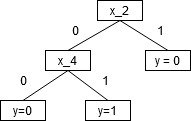
\includegraphics{cs5350hw1_1.jpg}
\item~
\newline Boolean function: $y=x_2' \wedge x_4$ 
\newline Table for function:
\begin{table}[h]
	\centering
	\begin{tabular}{cccc|c}
		$x_1$ & $x_2$ & $x_3$ & $x_4$ & $y$\\ 
		\hline\hline
		0 & 0 & 0 & 0 & 0 \\ \hline
		0 & 0 & 0 & 1 & 1 \\ \hline
		0 & 0 & 1 & 0 & 0 \\ \hline
		0 & 1 & 0 & 0 & 0 \\ \hline
		1 & 0 & 0 & 0.& 0\\ \hline
		0 & 0 & 1 & 1 & 1\\ \hline
		0 & 1 & 0 & 1 & 0\\ \hline
		0 & 1 & 1 & 0 & 0 \\ \hline
		1 & 0 & 0 & 1 & 1 \\ \hline
		1 & 0 & 1 & 0 & 0 \\ \hline
		1 & 1 & 0 & 0 & 0 \\ \hline
		0 & 1 & 1 & 1 & 0\\ \hline
		1 & 1 & 0 & 1 & 0\\ \hline
		1 & 0 & 1 & 1 & 1\\ \hline
		1 & 1 & 1 & 0 & 0\\ \hline
		1 & 1 & 1 & 1 & 0\\ \hline
	\end{tabular}
\end{table}

`\end{enumerate}
\item~ 
\begin{enumerate}
	\item~
	\newline First split:
	\newline -Outlook:
	\newline $S_s = 1, 2,8, 9, 11; p^+=2/5; Majority Error=.4$
	\newline $S_o=3, 7, 12, 13; p^+=4/4 = 1; Majority Error=0$
	\newline $S_r=4, 5, 6, 10, 14; p^+=3/5; Majority Error=.4$
	\newline $Information Gain=\frac{5}{14}-\frac{5}{14}\cdot (.4+.4)-\frac{4}{14} \cdot 0 = .07$
	\newline -Temperature:
	\newline $S_h = 1, 2, 3, 13; p^+=1/2; Majority Error=.5$
	\newline $S_m=4, 8, 10, 11, 12, 14; p^+=2/3; Majority Error=1/3$
	\newline $S_c=5, 6, 7, 9; p^+=3/4; Majority Error=.25$
	\newline $Information Gain=\frac{5}{14}-\frac{5}{14}\cdot (.5+.25)-\frac{6}{14} \cdot \frac{1}{3} = 0$
	\newline -Humidity:
	\newline $S_h = 1, 2, 3, 4, 8, 12, 14; p^+=3/7; Majority Error=3/7$
	\newline $S_n=5, 6, 7, 9, 10, 11, 13; p^+=6/7; Majority Error=1/7$
	\newline $S_l=none$
	\newline $Information Gain=\frac{5}{14}-\frac{7}{14}\cdot (\frac{3}{7}+\frac{1}{7}) = .07$
	\newline -Wind:
	\newline $S_s = 2, 6, 7, 11, 12, 14; p^+=1/2; Majority Error=.5$
	\newline $S_w=1, 3, 4, 5, 8, 9, 10, 13; p^+=3/4; Majority Error=.25$
	\newline $Information Gain=\frac{5}{14}-\frac{6}{14}\cdot (\frac{1}{2}-\frac{8}{14}) \cdot .25 = 0$
	\newline Outlook has the highest information gain so it will be used to split
	\newline
	\newline Second split of subsets:
	\newline Sunny subset 1, 2, 8, 9, 11:
	\newline -Temperature:
	\newline $S_h = 1, 2; p^+=0; Majority Error=0$
	\newline $S_m=8, 11, 14; p^+=1/2; Majority Error=.5$
	\newline $S_c=9; p^+=1; Majority Error=0$
	\newline $Information Gain=.4 \cdot \frac{2}{5} \cdot .5=.2$
	\newline -Humidity
	\newline $S_h = 1, 2, 8; p^+=0; Majority Error=0$
	\newline $S_n=9, 11; p^+=1; Majority Error=0$
	\newline $S_l=none$
	\newline $Information Gain=.4$
	\newline -Wind:
	\newline $S_s = 2,11; p^+=1/2; Majority Error=.5$
	\newline $S_w=1, 8, 9; p^+=1/3; Majority Error=\frac{1}{3}$
	\newline $Information Gain=.4-\frac{2}{5}\cdot.5-\frac{3}{5}\cdot\frac{1}{3} = 0$
	\newline Humidity has the largest information gain so it is used for the second split of the sunny subset of outlook
	\newline
	\newline The Humidity split has only two possible outcomes: 
	\newline $S_{sh}=1, 2, 8; p^+ =0$
	\newline $S_{sn}=9, 11; p^+ =1$
	\newline so this cannot be split anymore
	\newline
	\newline Overcast subset 3, 7, 12, 13:
	\newline For the overcast subset 3, 7, 12, 13; $p^+=1$ with Majority Error = 0, so this subset always results in 'yes'
	\newline
	\newline Rainy Subset 4, 5, 6, 10, 14:
	\newline -Temperature:
	\newline $S_h = none$
	\newline $S_m=4, 10, 14; p^+=2/3; Majority Error=.33$
	\newline $S_c=5, 6; p^+=1/2; Majority Error=.5$
	\newline $Information Gain=.4-\frac{3\cdot.33+2\cdot.5}{5}=0$
	\newline -Humidity
	\newline $S_h = 4, 14; p^+=1/2; Majority Error=.5$
	\newline $S_n=5, 6, 10; p^+=2/3; Majority Error=.33$
	\newline $S_l=none$
	\newline $Information Gain=.4-frac{2\cdot.5+3\cdot.33}{5}=0$
	\newline -Wind:
	\newline $S_s = 6, 14; p^+=0; Majority Error=0$
	\newline $S_w=4, 5, 10; p^+=1; Majority Error=0$
	\newline $Information Gain=.4$
	\newline Wind has the largest information gain from the rainy subset so it will be chosen to split. 
	\newline
	\newline The split subsets from the Rainy subset are:
	\newline $S_{rs}=6, 14; p^+=0; Majority Error = 0$
	\newline $S_{rw}=4, 5, 10; p^+=1; Majority Error = 0$
	\newline So the final result can be determined from this subset
	\newline
	\newline Final tree using Majority Error:
	\newline
	\newline 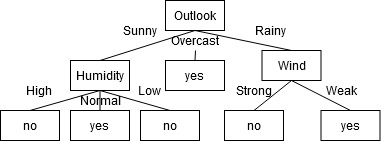
\includegraphics{cs5350hw1_2a.jpg}
	\item~
	\newline similar to part a above but using the Gini Index to calculate the information gain
	\newline First split:
	\newline -Outlook:
	\newline $S_s = 1, 2,8, 9, 11; p^+=2/5; Gini Index=.48$
	\newline $S_o=3, 7, 12, 13; p^+=4/4 = 1; Gini Index=0$
	\newline $S_r=4, 5, 6, 10, 14; p^+=3/5; Gini Index=.48$
	\newline $Information Gain=.46-\frac{5}{14}\cdot(.48+.48)=.12$
	\newline -Temperature:
	\newline $S_h = 1, 2, 3, 13; p^+=1/2; Gini Indexr=.5$
	\newline $S_m=4, 8, 10, 11, 12, 14; p^+=2/3; Gini Index=.44$
	\newline $S_c=5, 6, 7, 9; p^+=3/4; Gini Index=.38$
	\newline $Information Gain=.46-\frac{4\cdot.5+6\cdot.44+4\cdot.38}{14}=.02$
	\newline -Humidity:
	\newline $S_h = 1, 2, 3, 4, 8, 12, 14; p^+=3/7; Gini Index=.49$
	\newline $S_n=5, 6, 7, 9, 10, 11, 13; p^+=6/7; Gini Index=.24$
	\newline $S_l=none$
	\newline $Information Gain=.46\cdot\frac{7\cdot.49+7\cdot.24}{14} = .09$
	\newline -Wind:
	\newline $S_s = 2, 6, 7, 11, 12, 14; p^+=1/2; Gini Index=.5$
	\newline $S_w=1, 3, 4, 5, 8, 9, 10, 13; p^+=3/4;Gini Index=.38$
	\newline $Information Gain=.46\cdot\frac{6\cdot.5+8\cdot.38}{14} = .03$
	\newline Outlook has the highest information gain so it will be used to split
	\newline
	\newline Second split of subsets:
	\newline Sunny subset 1, 2, 8, 9, 11:
	\newline -Temperature:
	\newline $S_h = 1, 2; p^+=0; Gini Index=0$
	\newline $S_m=8, 11, 14; p^+=1/2; Gini Index=.5$
	\newline $S_c=9; p^+=1; Gini Index=0$
	\newline $Information Gain=.48-\frac{2}{5}\cdot.5=.28$
	\newline -Humidity
	\newline $S_h = 1, 2, 8; p^+=0; Gini Index=0$
	\newline $S_n=9, 11; p^+=1; Gini Index=0$
	\newline $S_l=none$
	\newline $Information Gain=.48$
	\newline -Wind:
	\newline $S_s = 2,11; p^+=1/2; Gini Index=.5$
	\newline $S_w=1, 8, 9; p^+=1/3; Gini Index=.44$
	\newline $Information Gain=.48-\frac{2}{5}\cdot.5-\frac{3}{5}\cdot.44=.02$
	\newline Humidity has the largest information gain so it is used for the second split of the sunny subset of outlook
	\newline
	\newline The Humidity split has only two possible outcomes: 
	\newline $S_{sh}=1, 2, 8; p^+ =0$
	\newline $S_{sn}=9, 11; p^+ =1$
	\newline so this cannot be split anymore
	\newline
	\newline Overcast subset 3, 7, 12, 13:
	\newline For the overcast subset 3, 7, 12, 13; $p^+=1$ with Gini Index = 0, so this subset always results in 'yes'
	\newline
	\newline Rainy Subset 4, 5, 6, 10, 14:
	\newline -Temperature:
	\newline $S_h = none$
	\newline $S_m=4, 10, 14; p^+=2/3; Gini Index=.44$
	\newline $S_c=5, 6; p^+=1/2; Gini Index=.5$
	\newline $Information Gain=.48-.6\cdot.44-.4\cdot.5=.16$
	\newline -Humidity
	\newline $S_h = 4, 14; p^+=1/2; Gini Index=.5$
	\newline $S_n=5, 6, 10; p^+=2/3; Gini Index=.44$
	\newline $S_l=none$
	\newline $Information Gain=.48-.4\cdot.5-.6\cdot.44=.16$
	\newline -Wind:
	\newline $S_s = 6, 14; p^+=0; Gini Index=0$
	\newline $S_w=4, 5, 10; p^+=1;Gini Index=0$
	\newline $Information Gain=.48$
	\newline Wind has the largest information gain from the rainy subset so it will be chosen to split. 
	\newline
	\newline The split subsets from the Rainy subset are:
	\newline $S_{rs}=6, 14; p^+=0; Gini Index = 0$
	\newline $S_{rw}=4, 5, 10; p^+=1; Gini Index = 0$
	\newline So the final result can be determined from this subset
	\newline
	\newline Final tree using Gini Index (Result is the same as part a):
	\newline
	\newline 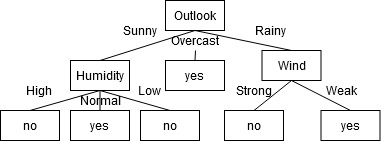
\includegraphics{cs5350hw1_2a.jpg}
	\item~
	\newline The trees from parts a and b are the same as the tree discussed in lecture. This is beacuse the algorithm always results in the same tree structure even if the information gain is calculated differently. Both the Majority Error and Gini Index functions work for this algorithm so the result should be the same. 
\end{enumerate}

\item~ 
\begin{enumerate}
\item~
\newline -Outlook:
	\newline $S_s = 1, 2,8, 9, 11, 15; p^+=1/2; Majority Error=1$
	\newline $S_o=3, 7, 12, 13; p^+ = 1; Majority Error=0$
	\newline $S_r=4, 5, 6, 10, 14; p^+=3/5; Majority Error=.97$
	\newline $Information Gain=.92-\frac{6\cdot1+4\cdot0+5\cdot.97}{15}=.197$
	\newline -Temperature:
	\newline $S_h = 1, 2, 3, 13; p^+=1/2; Majority Error=1$
	\newline $S_m=4, 8, 10, 11, 12, 14, 15; p^+=5/7; Majority Error=.86$
	\newline $S_c=5, 6, 7, 9; p^+=3/4; Majority Error=.81$
	\newline $Information Gain=.92-\frac{4+7\cdot.86+4\cdot.81}{15}=.04$
	\newline -Humidity:
	\newline $S_h = 1, 2, 3, 4, 8, 12, 14; p^+=3/7; Majority Error=.99$
	\newline $S_n=5, 6, 7, 9, 10, 11, 13, 15; p^+=7/8; Majority Error=.54$
	\newline $S_l=none$
	\newline $Information Gain=.92-\frac{7\cdot.99+8\cdot.54}{14}=.17$
	\newline -Wind:
	\newline $S_s = 2, 6, 7, 11, 12, 14; p^+=1/2; Majority Error=1$
	\newline $S_w=1, 3, 4, 5, 8, 9, 10, 13, 15; p^+=7/9; Majority Error=.76$
	\newline $Information Gain=.92-\frac{6\cdot1+9\cdot.76}{15}=.06$
	\newline
	\newline Outlook has the highest information gain, so it should be the chosen feature to split on. 
\item~
\newline -Outlook:
	\newline $S_s = 1, 2,8, 9, 11; p^+=.4; Majority Error=.97$
	\newline $S_o=3, 7, 12, 13, 15; p^+ = 1; Majority Error=0$
	\newline $S_r=4, 5, 6, 10, 14; p^+=3/5; Majority Error=.97$
	\newline $Information Gain=.92-\frac{5\cdot.97+5\cdot.97}{15}=.27$
	\newline -Temperature:
	\newline $S_h = 1, 2, 3, 13; p^+=1/2; Majority Error=1$
	\newline $S_m=4, 8, 10, 11, 12, 14, 15; p^+=5/7; Majority Error=.86$
	\newline $S_c=5, 6, 7, 9; p^+=3/4; Majority Error=.81$
	\newline $Information Gain=.92-\frac{4+7\cdot.86+4\cdot.81}{15}=.04$
	\newline -Humidity:
	\newline $S_h = 1, 2, 3, 4, 8, 12, 14; p^+=3/7; Majority Error=.99$
	\newline $S_n=5, 6, 7, 9, 10, 11, 13, 15; p^+=7/8; Majority Error=.54$
	\newline $S_l=none$
	\newline $Information Gain=.92-\frac{7\cdot.99+8\cdot.54}{14}=.17$
	\newline -Wind:
	\newline $S_s = 2, 6, 7, 11, 12, 14; p^+=1/2; Majority Error=1$
	\newline $S_w=1, 3, 4, 5, 8, 9, 10, 13, 15; p^+=7/9; Majority Error=.76$
	\newline $Information Gain=.92-\frac{6\cdot1+9\cdot.76}{15}=.06$
	\newline
	\newline Outlook still has the highest information gain, so it should be the chosen feature to split on.
\item~
\newline -Outlook:
	\newline $S_s = 1, 2,8, 9, 11, 15(\frac{5}{15}); p^+=\frac{2+5/14}{5+5/14}=.44; Majority Error=.99$
	\newline $S_o=3, 7, 12, 13, 15(\frac{4}{15}); p^+ = 1; Majority Error=0$
	\newline $S_r=4, 5, 6, 10, 14, 15(\frac{5}{15}); p^+=\frac{3+5/14}{5+5/14}=.63; Majority Error=.95$
	\newline $Information Gain=.92-\frac{5.36\cdot.99+5.36\cdot95}{15}=.23$
	\newline -Temperature:
	\newline $S_h = 1, 2, 3, 13; p^+=1/2; Majority Error=1$
	\newline $S_m=4, 8, 10, 11, 12, 14, 15; p^+=5/7; Majority Error=.86$
	\newline $S_c=5, 6, 7, 9; p^+=3/4; Majority Error=.81$
	\newline $Information Gain=.92-\frac{4+7\cdot.86+4\cdot.81}{15}=.04$
	\newline -Humidity:
	\newline $S_h = 1, 2, 3, 4, 8, 12, 14; p^+=3/7; Majority Error=.99$
	\newline $S_n=5, 6, 7, 9, 10, 11, 13, 15; p^+=7/8; Majority Error=.54$
	\newline $S_l=none$
	\newline $Information Gain=.92-\frac{7\cdot.99+8\cdot.54}{14}=.17$
	\newline -Wind:
	\newline $S_s = 2, 6, 7, 11, 12, 14; p^+=1/2; Majority Error=1$
	\newline $S_w=1, 3, 4, 5, 8, 9, 10, 13, 15; p^+=7/9; Majority Error=.76$
	\newline $Information Gain=.92-\frac{6\cdot1+9\cdot.76}{15}=.06$
	\newline
	\newline Outlook still has the highest information gain, so it should be the chosen feature to split on.
\item~
\newline Starting from the subsets to continue from part c:
\newline Sunny subset 1, 2, 8, 9, 11, $15(\frac{5}{14})$:
\newline -Temperature:
	\newline $S_h = 1, 2; p^+=0; Majority Error=0$
	\newline $S_m=8, 11, 15(\frac{5}{14}); p^+=\frac{1+5/14}{2+5/14}=.58; Majority Error=.98$
	\newline $S_c=9; p^+=1; Majority Error=0$
	\newline $Information Gain=.99-\frac{2.36\cdot.98}{5.36}$
	\newline -Humidity
	\newline $S_h = 1, 2, 8; p^+=0; Majority Error=0$
	\newline $S_n=9, 11, 15(\frac{5}{14}); p^+=1; Majority Error=0$
	\newline $S_l=none$
	\newline $Information Gain=.99$
	\newline -Wind:
	\newline $S_s = 2,11; p^+=1/2; Majority Error=1$
	\newline $S_w=1, 8, 9, 15(\frac{5}{14}); p^+=\frac{1+5/14}{3+5/14}=.4; Majority Error=.97$
	\newline $Information Gain=.99-\frac{2\cdot1+3.36\cdot.97}{5.36}=.009$
	\newline Humidity has the largest information gain so it is used for the second split of the sunny subset of outlook
	\newline
	\newline The Humidity split has only two possible outcomes: 
	\newline $S_{sh}=1, 2, 8; p^+ =0$
	\newline $S_{sn}=9, 11; p^+ =1$
	\newline so this cannot be split anymore
	\newline
	\newline Overcast subset 3, 7, 12, 13, $15(\frac{4}{15})$:
	\newline For the overcast subset 3, 7, 12, 13, $15(\frac{4}{15})$; $p^+=1$ with Majority Error = 0, so this subset always results in 'yes'
	\newline
	\newline Rainy Subset 4, 5, 6, 10, 14, $15(\frac{5}{15})$:
	\newline -Temperature:
	\newline $S_h = none$
	\newline $S_m=4, 10, 14, 15(\frac{5}{15}); p^+=\frac{2+5/14}{3+5/14}=.7; Majority Error=.88$
	\newline $S_c=5, 6; p^+=1/2; Majority Error=1$
	\newline $Information Gain=.95-\frac{3.36\cdot.88+2}{5.36}=.03$
	\newline -Humidity
	\newline $S_h = 4, 14; p^+=1/2; Majority Error=1$
	\newline $S_n=5, 6, 10, 15(\frac{5}{14}); p^+=\frac{2+5/14}{3+5/14}=.44; Majority Error=.88$
	\newline $S_l=none$
	\newline $Information Gain=.95-\frac{2+3.36\cdot.99}{5.36}=.03$
	\newline -Wind:
	\newline $S_s = 6, 14; p^+=0; Majority Error=0$
	\newline $S_w=4, 5, 10, 15(\frac{5}{14}); p^+=1; Majority Error=0$
	\newline $Information Gain=.95$
	\newline Wind has the largest information gain from the rainy subset so it will be chosen to split. 
	\newline
	\newline The split subsets from the Rainy subset are:
	\newline $S_{rs}=6, 14; p^+=0; Majority Error = 0$
	\newline $S_{rw}=4, 5, 10; p^+=1; Majority Error = 0$
	\newline So the final result can be determined from this subset
	\newline
	\newline Final tree for part d:
	\newline
	\newline 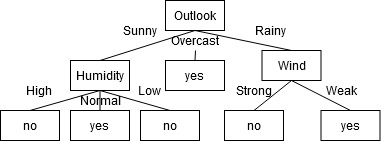
\includegraphics{cs5350hw1_2a.jpg}

\end{enumerate}
\item ~[\textbf{Bonus question 1}]~[5 points].  Prove that the information gain is always non-negative.  That means, as long as we split the data, the purity will never get worse! (Hint: use convexity)
\item ~[\textbf{Bonus question 2}]~[5 points].  We have discussed how to use decision tree for regression (i.e., predict numerical values) --- on the leaf node, we simply use the average of the (numerical) labels as the prediction.  Now, to construct a regression tree, can you invent a gain to select the best attribute to split data in ID3 framework?

\end{enumerate}

\section{Decision Tree Practice [60 points]}
\begin{enumerate}
	\item~[5 Points] Starting from this assignment, we will build a light-weighted machine learning library. 
To this end, you will first need to create a code repository in \href{https://github.com/}{Github.com}. Please refer to the short introduction in the appendix and the \href{https://guides.github.com/activities/hello-world/}{official tutorial} to create an account and repository. Please commit a README.md file in your repository, and write one sentence: "This is a machine learning library developed by \textbf{Your Name} for CS5350/6350 in University of Utah".  You can now create a first folder, "DecisionTree". Please leave the link to your repository in the homework submission. We will check if you have successfully created it. 


\item~[30 points] We will implement a decision tree learning algorithm for car evaluation task. The dataset is from UCI repository(\url{https://archive.ics.uci.edu/ml/datasets/car+evaluation}). Please download the processed dataset (car.zip) from Canvas.  In this task, we have $6$ car attributes, and the label is the evaluation of the car. The attribute and label values are listed in the file ``data-desc.txt". All the attributes are categorical.  The training data are stored in the file ``train.csv'', consisting of $1,000$ examples. The test data are stored in ``test.csv'', and comprise $728$ examples. In both training and test datasets, attribute values are separated by commas; the file ``data-desc.txt''  lists the attribute names in each column. 
\\

\noindent Note: we highly recommend you to use Python for implementation, because it is very convenient to load the data and handle strings. For example, the following snippet reads the CSV file line by line and split the values of the attributes and the label into a list, ``terms''. You can also use ``dictionary'' to store the categorical attribute values. In the web are numerous tutorials and examples for Python. if you have issues, just google it!
\begin{lstlisting}
with open(CSVfile, 'r') as f:
     for line in f:
            terms = line.strip().split(',')
            process one training example
\end{lstlisting}
\begin{enumerate}
\item~[15 points] Implement the ID3 algorithm that supports, information gain,  majority error and gini index to select attributes for data splits. Besides, your ID3 should allow users to set the maximum tree depth. Note: you do not need to convert categorical attributes into binary ones and your tree can be wide here. 
\item~[10 points] Use your implemented algorithm to learn decision trees from the training data. Vary the maximum  tree depth from $1$ to $6$  --- for each setting, run your algorithm to learn a decision tree, and use the tree to  predict both the training  and test examples. Note that if your tree cannot grow up to 6 levels, then you can stop at the maximum level. Report in a table the average prediction errors on each dataset when you use information gain, majority error and gini index heuristics, respectively.

\item~[5 points] What can you conclude by comparing the training errors and the test errors? 
\end{enumerate}


\item~[25 points] Next, modify your implementation a little bit to support numerical attributes. We will use a simple approach to convert a numerical feature to a binary one. We choose the media (NOT the average) of the attribute values (in the training set) as the threshold, and examine if the feature is bigger (or less) than the threshold. We will use another real dataset from UCI repository(\url{https://archive.ics.uci.edu/ml/datasets/Bank+Marketing}). This dataset contains $16$ attributes, including both numerical and categorical ones. Please download the processed dataset from Canvas (bank.zip).  The attribute and label values are listed in the file ``data-desc.txt". The training set is the file ``train.csv'', consisting of $5,000$ examples, and the test  ``test.csv'' with $5,000$ examples as well.  In both training and test datasets, attribute values are separated by commas; the file ``data-desc.txt''  lists the attribute names in each column. 
\begin{enumerate}
	\item~[10 points] Let us consider ``unkown'' as a particular attribute value, and hence we do not have any missing attributes for both training and test. Vary the maximum  tree depth from $1$ to $16$ --- for each setting, run your algorithm to learn a decision tree, and use the tree to  predict both the training  and test examples. Again, if your tree cannot grow up to $16$ levels, stop at the maximum level. Report in a table the average prediction errors on each dataset when you use information gain, majority error and gini index heuristics, respectively.
	
	\item~[10 points] Let us consider "unkown" as  attribute value missing. Here we simply complete it with the majority of other values of the same attribute in the training set.   Vary the maximum  tree depth from $1$ to $16$ --- for each setting, run your algorithm to learn a decision tree, and use the tree to  predict both the training  and test examples. Report in a table the average prediction errors on each dataset when you use information gain, majority error and gini index heuristics, respectively.
	
	
	\item~[5 points] What can you conclude by comparing the training errors and the test errors, with different tree depths, as well as different ways to deal with "unkown" attribute values?
\end{enumerate}
\end{enumerate}

\section*{Appendix}
\section*{What is GitHub?}
You may have contacted with GitHub long before you realized its existence, since a large part of open source code reside in GitHub nowadays. And whenever you google for some open source code snap, like code for a course project or a research paper, you would possibly be directed to GitHub. 

GitHub, as well as  many of its competitor like GitLab and BitBucket, is a so-called code hosting website, to which you upload and manage your code. For many first time user of GitHub, it's quite confusing that there is another software called git. Don't be confused now, git is a version control software and is the core of all these website. It can help you track the development of your code and manage them in a very organized way. Git works on your own local computer as other normal softwares do. Github, however, is just a website, or by its name, a hub, that you keep the code, just like a cloud storage space. How do we upload our code to GitHub? Yes, by Git!( or its variants). They are so dependent that when people say using GitHub, they mean they use git to manage their code, and keep their code in GitHub. That been said, as a stand-alone tool, git could  work perfectly on your local computer without Internet access, as long as your do not want to keep your code on-line and access them everywhere, or share them with others. 



\section*{Core concepts and operations of GitHub}
Here we only state the basic concepts of GitHub and git. Specific commands vary slightly depending on the Platforms ( Mac/Linux/WIN10) and command-line/GUI versions. Please refer to the link provided below for concrete examples and video tutorials. As you understand the whole working flow, those commands should be easy and straightforward to use. 

There are two major parts we need to know about github. The on-line part of GitHub and local part of git. We start from GitHub.

\subsection*{GitHub}
If you have never had a GitHub account, please follow this link to create one. It also provides tutorial on basic operations of GitHub.


\href{https://guides.github.com/activities/hello-world/}{https://guides.github.com/activities/hello-world/}\\

Note that now you can create a private repository without paying to GitHub. In principle, we encourage you to create public repository. But if you somehow prefer a private one( i.e., can't be access by others), you must add TA's account as the collaborators in order to check your work.  

These are some key concept you should know about:
\begin{itemize}
	\item Repository: Repository is the place where you keep your whole project, including every version, every branch of the code. For example, you will need to create a repository named Final-Project (or other suitable name), which will contain all your code, report and results.
	
	\item Branch: Branch allows you (and your partners) to developed different version of a repository at the same time. For example, you and your partner are working on the final project. Suddenly, you want to try some crazy algorithm but not sure if it would work. Now you create a new branch of the repository and continue your trying without breaking the original (usually called master) branch. If successful, you then merge this branch with the master branch. Otherwise, you can simply give up and delete this branch, and nothing in the master branch will be affected. 
	
	\item Pull Request: This is the heart of GitHub. Don't mistake this with PULL we will talk about later. Pull Request means when you finish your branch( like the crazy algorithm above), you make a request that the owner or manager of master branch to review your code, and merge them into the master branch. If accepted, any changes you make in your branch will also be reflected in the master branch. As the manager of master branch, you should also be careful to check the code about to be merged and address any potential conflicts this merge may introduce. 
	
	\item Merge: This operation means to merge two different branches into a single one. Any inconsistency must be addressed before merging. 
\end{itemize}

\subsection*{git}


This link provides installation guides and video tutorial for basic git operation.

\href{https://git-scm.com/doc}{https://git-scm.com/doc}\\

This is a cheating-sheet for common commands of git.

\href{https://confluence.atlassian.com/bitbucketserver/basic-git-commands-776639767.html}{https://confluence.atlassian.com/bitbucketserver/basic-git-commands-776639767.html}\\

As said before, you can always use git in a local repository. More frequently, we link this repository to the one you create in GitHub and then you can use git to push (upload) you code to and pull (fetch) them from GitHub. Beside the original command-line interface, there are many softwares with nice GUI to access the functionalities of git, such as GitHub Desktop and Source Tree. 


There are also some core operations you should know about:
\begin{itemize}
	\item clone: Download/Copy a repository from GitHub to your local disk. This would fetch everything of this repository. This is the most commonly used command to download someone else's code from GitHub.
	
	\item init: Initialize current fold a to local repository, which will generate some hidden files to track the changes.
	
	\item add: By default, no files in the repository folder are marked to be tracked. When you want to track the change of a file, use add operation to add this file to the tracking list. Normally, we only track the source code and report of our project, and we DON'T track datasets. As the datasets  never change once downloaded and are usually big. 
	
	\item commit: This is the most frequently used git operation. Commit means to make a LOCALLY check point. For example, you have done some change to the project, like adding a new  complex function, and it works well. Then you can commit with a comment "adding new function, test well ***". Later when you try to modify this function but fail, you can roll back to this check point and start over. Hence you do not need to  many copies before modification. 
	
	\item checkout: After you commit checkpoints, you can use checkout to roll back to these checkpoints in case you mess up.
	
	\item push: When you complete current task and make check very thing is good, you use push( after commit) to upload the local repository to GitHub. 
	
	\item pull: Fetch the content from GitHub. This is similar to Clone. But it only fetches content designated by the  parameters to the pull command.    
\end{itemize}

\subsection*{Work Flow}
With concepts and operations introduced above, the work flow of using GitHub for a project is as follows:
\begin{enumerate}
	\item Create a repository in GitHub.
	\item Create a local repository in your local computer and link it to the remote repository in GitHub.
	\item Create source code files and add them to the tracking list.
	\item Edit, modify and test your code. Commit and checkout whenever mess up.
	\item Push your code to GitHub.
\end{enumerate}

If you start your work with an existed GitHub repository (like  the one created by your partner), Just replace steps 1 to 3 by pull or clone. \\

You can play around with GitHub by creating some random  repositories and files to track. 
Basic operation introduced above and in the links are more than enough to complete this course. If are you have further interest to master GitHub, there are several excellent on-line courses provided by Coursera and Udacity. Many tutorials are provided in the web as well. 


\end{document}
%%% Local Variables:
%%% mode: latex
%%% TeX-master: t
%%% End:
